%%%%%%%%%%%%%%%%%%%%%%%%%%%%%%%%%%%%%%%%%%%%%%%%%%%%%%%%%%%%%%%%%%%%%%%%%%%%%%%%
%%%%%%%%%%%%%%%%%%%%%%%%%%%%%%%%%%%%%%%%%%%%%%%%%%%%%%%%%%%%%%%%%%%%%%%%%%%%%%%%
%%                                                                            %%
%% opintnaytepohja.tex versio 3.20 (2018/08/31)                               %%
%% Opinnäytepohja käytettäväksi aaltothesis.sty (versio 3.20) -tyylitiedoston %%
%% kanssa.                                                                    %%
%% Toimiakseen paketti tarvitsee pdfx.sty v. 1.5.84 (2017/05/18) tai uudempi. %% 
%% The LaTeX template file to be used with the aaltothesis.sty (version 3.20) %%
%% style file.                                                                %%
%% This package requires pdfx.sty v. 1.5.84 (2017/05/18) or newer.            %% 
%%                                                                            %%
%% This is licensed under the terms of the MIT license below.                 %%
%%                                                                            %%
%% Written by Luis R.J. Costa.                                                %%
%% Currently developed at the Learning Services of Aalto University School of %%
%% Electrical Engineering by Luis R.J. Costa since May 2017.                  %%
%%                                                                            %%
%% Copyright 2017-2018, by Luis R.J. Costa, luis.costa@aalto.fi,              %%
%% Copyright 2017-2018 Swedish translations in aaltothesis.cls by Elisabeth   %%
%% Nyberg, elisabeth.nyberg@aalto.fi and Henrik Wallén,                       %%
%% henrik.wallen@aalto.fi.                                                    %%
%% Copyright 2017-2018 Finnish documentation in the template opinnatepohja.tex%%
%% by Perttu Puska, perttu.puska@aalto.fi, and Luis R.J. Costa.               %%
%% Copyright 2018 English template thesistemplate.tex by Luis R.J. Costa.     %%
%% Copyright 2018 Swedish template kandidatarbetsbotten.tex by Henrik Wallen. %%
%%                                                                            %%
%% Permission is hereby granted, free of charge, to any person obtaining a    %%
%% copy of this software and associated documentation files (the "Software"), %%
%% to deal in the Software without restriction, including without limitation  %%
%% the rights to use, copy, modify, merge, publish, distribute, sublicense,   %%
%% and/or sell copies of the Software, and to permit persons to whom the      %%
%% Software is furnished to do so, subject to the following conditions:       %%
%% The above copyright notice and this permission notice shall be included in %%
%% all copies or substantial portions of the Software.                        %%
%% THE SOFTWARE IS PROVIDED "AS IS", WITHOUT WARRANTY OF ANY KIND, EXPRESS OR %%
%% IMPLIED, INCLUDING BUT NOT LIMITED TO THE WARRANTIES OF MERCHANTABILITY,   %%
%% FITNESS FOR A PARTICULAR PURPOSE AND NONINFRINGEMENT. IN NO EVENT SHALL    %%
%% THE AUTHORS OR COPYRIGHT HOLDERS BE LIABLE FOR ANY CLAIM, DAMAGES OR OTHER %%
%% LIABILITY, WHETHER IN AN ACTION OF CONTRACT, TORT OR OTHERWISE, ARISING    %%
%% FROM, OUT OF OR IN CONNECTION WITH THE SOFTWARE OR THE USE OR OTHER        %%
%% DEALINGS IN THE SOFTWARE.                                                  %%
%%                                                                            %%
%%                                                                            %%
%%%%%%%%%%%%%%%%%%%%%%%%%%%%%%%%%%%%%%%%%%%%%%%%%%%%%%%%%%%%%%%%%%%%%%%%%%%%%%%%
%%                                                                            %%
%%                                                                            %%
%% Esimerkki opinnäytteen tekemisestä LaTeX:lla                               %%
%% Alkuperäinen versio ja nykinen kehitystyö Luis Costa, muutokset            %%
%% suomenkieliseen tekstipohjaan Perttu Puska.  							  %%
%% Tämän version on systeemianalyysin kanditöihin sopivaksi muokannut Juho    %%
%% Roponen.	Uutena lisätty mm. fiplainnat.bst, joka mahdollistaa              %%
%% suomenkielisten lähteiden kätevän käsittelyn .bib-tiedostolla. 			  %%
%% Ruotsinkielen tuki lisätty 15092014                                        %%
%% PDF/A-1b -tuki lisätty 15092017                                            %%
%% PDF/A-2b -tuki lisätty 24042018                                            %%
%%                                                                            %%
%% Tähän esimerkkiin kuuluu tiedostot                                         %%
%%        opinnaytepohja.tex (versio 3.20) (suomenkielinen pohja)             %%
%%        thesistemplate.tex (versio 3.20) (for text in English)              %%
%%        kandidatarbetsbotten.tex (versio 1.00) (ruotsinkielinen kandipohja) %%
%%        aaltothesis.cls (versio 3.20)                                       %%
%%        linediagram.eps                                                     %%
%%        curves.eps                                                          %%
%%        linediagram.pdf                                                     %%
%%        curves.pdf                                                          %%
%%        ledspole.jpg                                                        %%
%%                                                                            %%
%%                                                                            %%
%% Kääntäminen Linuxissa joko                                                 %%
%% pdflatex: (suositeltava tapa)                                              %%
%%             $ pdflatex opinnaytepohja                                      %%
%%             $ pdflatex opinnaytepohja                                      %%
%%                                                                            %%
%%   Tuloksena on tiedosto opinnaytepohja.pdf, joka on PDF/A-standardin       %%
%%   mukainen, jos olet valinnut oikeat \documentclass -optiot (kts. alla) ja %%
%%   ja käyttämäsi kuvatiedostoissa ei ole ongelmia.                          %%
%%                                                                            %%
%% Tai                                                                        %%
%% latex: (ei ole suositeltava tapa)                                          %%
%%             $ latex opinnaytepohja                                         %%
%%             $ latex opinnaytepohja                                         %%
%%                                                                            %%
%%   Tuloksena on tiedosto opinnayte.dvi, joka muutetaan ps-muotoon           %%
%%   seuraavasti                                                              %%
%%                                                                            %%
%%             $ dvips opinnaytepohja -o                                      %%
%%                                                                            %%
%%   ja edelleen pdf-muotoon seuraavasti                                      %%
%%                                                                            %%
%%             $ ps2pdf opinnaytepohja.ps                                     %%
%%                                                                            %%
%%   Tämä pdf EI ole pdf/a -tiedosto vaan se pitää muuttaa sellaiseksi esim.  %%
%%   Acrobat Pro- tai PDF-XChange -ohjelmalla.                                %%
%%                                                                            %%
%%                                                                            %%
%% Selittävät kommentit on tässä esimerkissä varustettu %%-merkeillä ja       %%
%% muutokset, joita käyttäjä voi tehdä, on varustettu %-merkeillä             %%
%%                                                                            %%
%%%%%%%%%%%%%%%%%%%%%%%%%%%%%%%%%%%%%%%%%%%%%%%%%%%%%%%%%%%%%%%%%%%%%%%%%%%%%%%%
%%%%%%%%%%%%%%%%%%%%%%%%%%%%%%%%%%%%%%%%%%%%%%%%%%%%%%%%%%%%%%%%%%%%%%%%%%%%%%%%
%%
%% MIKÄ on PDF/A?
%%
%% PDF/A on ISO-standardoitu versio pdf-tiedostosta. Standardin tavoite on, että
%% tiedosto on toistettavissa myös pitkänkin ajan kuluessa. PDF/A eroaa pdf:stä
%% siinä, että se sallii vain sellaisia pdf-ominaisuuksia, jotka tukevat
%% tiedoston pitkäaikaista arkistointia. Esim. PDF/A vaati, että kaikki käytetyt
%% fontit ovat mukana tiedostossa, mutta tavallisessa pdf:ssä voi olla niin,
%% että tiedostossa on vain linkki tiedostonlukijan tietokonejärjestelmän
%% fontteihin. PDF/A vaatii myös tietoa mm. värimäärittelystä ja käytetystä
%% salauksesta.
%% Tällä hetkellä PDF/A standardeja on kolme:
%% PDF/A-1: perustana PDF 1.4, standardi ISO19005-1, julkaistu vuonna 2005.
%%          Kaikki perusvaatimukset pitkäaikaiseen arkistointiin käytössä.
%% PDF/A-2: perustana PDF 1.7, standardi ISO19005-2, julkaistu vuonna 2011.
%%          Yllä olevan lisäksi tukee mm. OpenType-fonttien sisällyttämistä,
%%          läpinäkyvyyttä värimäärittelyssä ja digitaalisia allekirjoituksia.
%% PDF/A-3: perustana PDF 1.7, standardi ISO19005-3, julkaistu vuonna 2012.
%%          Eroaa edellisestä ainoastaan siinä, että se sallii missä tahansa
%%          tiedostoformaatissa (esim. xml, csv, cad, taulukkolaskentaformaatit,
%%          tekstinkäsittelyformaatit) olevien tiedostojen sisällyttämisen.
%% PDF/A-1 tiedostot eivät välttämättä ole PDF/A-2 -yhteensopivia eikä PDF/A-2
%% tiedostot ole PDF/A-1 -yhteensopivia.
%% Kaikista yllä olevista PDF/A-standardeista on kaksi tasoa:
%% b: (basic) vaatii, että tiedoston visuaalinen ilme on luotettavasti
%%    toistettavissa.
%% a: (accessible) b-tason vaatimuksien lisäksi, määrittelee kuinka saavutettava
%%    pdf-tiedosto on mm. vammaisteknologiaa hyödynttävissä ohjelmistoissa 
%%    (esim. kosketusruutua käytettävissä laitteissa).
%% Lisätietoa PDF/A:sta esim. https://en.wikipedia.org/wiki/PDF/A tai 
%%
%%
%% MINKÄ PDF/A -standardin mukaan teen opinnäytetyöni?
%%
%% Ensisijaisesti PDF/A-1b -standardin mukaan. Kuvaajat ja kuvat mitä
%% tyypillisesti käytetään opinnäytetyössä eivät tarvitse
%% läpinäkyvyysominaisuuksia. Perus '2D' -näkymä on riittävä. Opinnäytetyössä
%% käytettävät fontit on määritelty tässä pohjassa eikä niitä pidä muuttaa. Jos
%% käytät kuvia, jossa läpikäkyvyysominaisuuksillä on merkitystä, käytä PDF/A-2b
%% -standardia. Älä käytä PDF/A-3b -standardia opinnäytetyössäsi.
%%
%%
%% MITKÄ kuvaformaatteja voin käyttää PDF/A-tiedoston tekemisessä?
%%
%% Kun käytät pdflatexia työsi kääntämisessä suosi pdf-formaattia, mutta voit
%% käytä myös jpg- ja/tai png-formmaatia eteenkin valokuvissa.
%% Pdf-muotoisten kuvien kanssa voi tulla ongelmia PDF/A -yhteesopivuuden
%% kanssa, mm. jos fontit eivät ole upotettu tiedostoon.
%% Älä käytä PDF/A-formaattia kuvatiedostoissa.
%% Jos kuitenkin käytät perus latexia työsi kääntämisessä, ainoa sallittu
%% kuvaformaatti on eps. ÄLÄ käytä ps-formaattia kuvissasi.
%%
%% KÄYTÄ näistä yhtä:
%% * ensimmäinen, jos käytät pdflatexia, joka kääntää tekstin suoraan
%%   pdf/a-tiedostoksi ja haluat julkaista opinnäytetyösi verkossa
%% * toinen, jos haluat tulostaa opinnäytteesi kansitettavaksi
%% * kolmas jos haluat tuottaa ps-tiedostoa ja siitä pdf/a:ta
%%
%\documentclass[finnish, 12pt, a4paper, sci, utf8, a-1b, online]{aaltothesis}
%\documentclass[finnish, 12pt, a4paper, elec, utf8, a-1b]{aaltothesis}
%\documentclass[finnish, 12pt, a4paper, elec, dvips, online]{aaltothesis}
%%
%% Kirjoita y.o. \documentclass optioiksi
%% * korkeakoulusi näistä: arts, biz, chem, elec, eng, sci
%% * editorisi käyttämä merkkikoodaustapa: utf8, latin1
%% * opinnäytetyön kieli: finnish, english, swedish
%% * tee arkistointikelpoista PDF/A-1b tai PDF/A-2b pdf-tiedosto: a-1b, a-2b
%%                         (pdflatex tuottaa tavallisen metadataa sisältävän
%%                          pdf-tiedoston ilman a-*b optiota)
%% * verkkoon menevä symmetrinen taitto, sinisellä hypertekstillä: online  
%%                         (oletusarvo on leveä marginaali sivun sidonta
%%                          puolella ja musta hyperteksti)
%% * kaksipuolinen tulostus: twoside (oletusarvo on yksipuolinen tulostus)
%%

%% Käytä yhtä näistä, jos kirjoitat englanniksi. Katso englanninokset
%% tiedostosta thesistemplate.tex.
\documentclass[english, 12pt, a4paper, sci, utf8, a-1b, online]{aaltothesis}
%\documentclass[english, 12pt, a4paper, elec, utf8, a-1b]{aaltothesis}
%\documentclass[english, 12pt, a4paper, elec, dvips, online]{aaltothesis}

%% Jos kirjoitat ruotsiksi, katso kandidatarbetsbotten.tex ruotsinskielistä
%% kandipohjaa.
%\documentclass[swedish, 12pt, a4paper, elec, utf8, a-1b, online]{aaltothesis}
%\documentclass[swedish, 12pt, a4paper, elec, utf8, a-1b]{aaltothesis}
%\documentclass[swedish, 12pt, a4paper, elec, dvips, online]{aaltothesis}


\usepackage{graphicx}
\usepackage{algpseudocode} 
\usepackage{algorithm} 

%% Matematiikan fontteja, symboleja ja muotoiluja lisää, näitä tarvitaan usein
\usepackage{amsfonts, amssymb, amsbsy, amsmath}
\usepackage[english]{babel}
\usepackage{natbib}
\usepackage{subfigure}
\usepackage{pgfplots}

\newpage
%\bibliographystyle{fiplainnat}
\bibliographystyle{plainnat}

\setcitestyle{authoryear,open={(},close={)}}
\usepackage{tikz}
\usetikzlibrary{arrows, positioning, shapes.geometric, shapes,snakes}
\usepackage{float}
\usepackage{booktabs}
\usepackage{adjustbox}
%% Korjaa vastaamaan korkeakouluasi, jos automaattisesti asetettu nimi on
%% virheellinen. Annettu korkeakoulun nimi ei tule Aalto-logoon.
%%
%% Change the school field to specify your school if the automatically set name
%% is wrong. The specified school name will not be contained in the Aalto logo.
% \school{Korkeakouluni}

%% Korjaa seuraavat vastaamaan koulutusohjelmaasi
%%
\degreeprogram{Engineering Physics and Mathematics}
%%

%% Pääaineesi
\major{Mathematics and Operations Research}

%% Pääainekoodi
%%
\code{SCI3029}
%%

%% 
%% Valitse yksi näistä kolmesta
%%
\univdegree{BSc}
%\univdegree{MSc}
%\univdegree{Lic}
%%

%% Oma nimi
%%
\thesisauthor{Pietari Kaskela}
%%

%% Opinnäytteen otsikko tulee tähän ja mahdollisesti uudelleen englannin- tai
%% ruostinkielisen abstraktin yhteydessä. Älä tavuta otsikkoa ja vältä liian
%% pitkää otsikkotekstiä. Jos LaTeX ryhmittelee otsikon huonosti, voit joutua
%% pakottamaan rivinvaihdon \\ -kontrollimerkillä.
%% Tällöin...
%% Muista että otsikkoja ei tavuteta! 
%% Jos otsikossa on ja-sana, se ei jää rivin viimeiseksi sanaksi vaan aloittaa
%% uuden rivin.
%% Anna ostikko uudelleen ilman rivinvaihtomerkkiä optionaalisena argumenttina
%% hakasuluissa. Näin tehdään, koska otsikko on osaa pdf/a-tiedostossa olevaa
%% metadataa, ja metadatassa ei saa olla rivinvaihtomerkkiä.
%%
\thesistitle{Optimizing preprocessing and local search heuristics of the traveling salesman problem with parallel programming}
%\thesistitle[Opinnäytteen otsikko]{Opinnäyteen\\ otsikko}
%%

%%
\place{Espoo}
%%

%% Kandidaatintyön päivämäärä on sen esityspäivämäärä! 
%% 
\date{6.12.2020}
%%

%% Kandidaatin- tai diplomityön valvoja.
%% Huomaa tittelissä "\" -merkki pisteen jälkeen, ennen välilyöntiä ja
%% seuraavaa merkkijonoa. 
%% Näin kerrotaan LaTeXille, että kyseessä ei ole lauseen loppu, jonka jälkeen
%% tulee hieman pidempi väli vaan halutaan tavallinen väli.
%%
\supervisor{Prof. Fabricio Oliveira}
%%

%% Kandidaatintyön ohjaaja(t) tai diplomityön ohjaaja(t). Ohjaajia saa olla
%% korkeintaan kaksi.
%% 
\advisor{MSc (Tech.) Juho Andelmin}
%\advisor{DI Tina Tutkija}
%%

%% Aaltologo: syntaksi:
%% \uselogo{aaltoRed|aaltoBlue|aaltoYellow|aaltoGray|aaltoGrayScale}{?|!|''}
%% Logon kieli on sama kuin dokumentin kieli
%%
\uselogo{aaltoBlack}{''}

%%

%% Suomenkielinen tiivistelmä:
%% Kaikki tiivistelmässä tarvittava tieto (nimesi, työnnimi, jne.) käytetään
%% niin kuin se on yllä määritelty.
%% Tiivistelmän avainsanat:
%% Huom! Avainsanat erotetaan toisistaan \spc -makrolla
%%
\keywords{Traveling salesman\spc TSP\spc CUDA\spc Parallel programming\spc 2-opt\spc alpha-nearness}
%%

%% Tiivistelmän tekstiosa. Tämä teksti sisältyy pdf-tiedoston metadataa ja tulee
%% myös tiivistelmälomakkeeseen.
%%
\thesisabstract{
This thesis aims to optimize algorithms for solving the traveling salesman problem (TSP) with parallel programming. The traveling salesman problem is about finding the shortest possible route, which visits all of the given cities, returning to the starting city. The problem is NP-hard, which means that there are no fast exact algorithms for solving the problem. However, inexact heuristic solution methods work very well in practice and are capable of producing near optimal solutions for large problem instances. The heuristic TSP solver implemented in this thesis first preprocesses the input graph to identify those edges, which most likely belong to the shortest route. The identification is done with $\alpha$-values, which have been empirically verified to produce good candidate edges. The generated set of candidate edges is then used to form a number of initial routes, which are then improved with local heuristic algorithms. The most computationally heavy parts of the algorithms are implemented using CUDA parallel programming language. CUDA allows the distribution of the workload to thousands of parallel threads in graphics processing units (GPUs). The optimization of $\alpha$-values in graph preprocessing achieves a speedup of up to 10 times compared to a normal implementation, by parallelizing the minimum spanning tree calculation. Parallel programming is also applied to the 2-opt heuristic, which achieves speedups of up to 10-40 times, compared to a normal implementation. The effectiveness of combining these parallel implementations into a full solver is demonstrated by obtaining competitive results in solving a set of benchmark instances from TSPLIB. The developed implementations are also easily generalizable to n-dimensional problem instances with different metrics.
}
%%

%% Tekijänoikeusteksti. Tekijänoikeus on tekijällä riippumatta siitä onko
%% copyright -merkintä näkyvissä vai ei. Halutessasi voit jakaa työsi Creative
%% Commons -lisensillä (katso creativecommons.org), jolloin lisenssitekstin on
%% oltava näkyvissä. Kirjoita tähän haluamasi tekijänoikeustektin. Se kirjautuu
%% myös pdf-tiedoston metadataan.
%% Syntaksi:
%% \copyrigthtext{metadatateksti}{sivulle näkyviin tuleva teksti}
%%
%% A.o. metadataan menevässä tekstissä on käytettävä \noexpand -makroa ennen
%% \copyright -erikoismerkkiä ja lisäksi makrot (tässä \copyright ja \year) on
%% erotettava seuraavasta tekstistä \ -merkillä (välilyöntimerkki).
%% \copyrighttext-makron argumentissa olevat makrot automaattisesti hakevat
%% vuosiluvun ja tekijän nimi.
%% (Huom! \ThesisAuthor on aaltothesis.cls -tyylitiedoston sisäinen makro).
%% Toki saman tekstin olisi voinut kirjoittaa yksinkertaisesti näin:
%% \copyrighttext{Copyright \noexpand\copyright\ 2018 Teemu Teekkari}
%% {Copyright \copyright{} 2018 Teemu Teekkari}
%%
\copyrighttext{Copyright \noexpand\copyright\ \number\year\ \ThesisAuthor}
{Copyright \copyright{} \number\year{} \ThesisAuthor 
\\\\The document can be stored and made available to the public on the open internet pages of Aalto University.\\
All other rights are reserved.
}
%% Jos et halua työtäsin näkyviin systislabran verkkosivuille, poista 
%% copyright noticesta lupa jakaa työ Aallon verkkosivuilla.
%%

%% Voit estää LaTeXia kirjoittamasta xmpdata-tiedostoon (sisältää pdf
%% -tiedostoon kirjoitettavaa metadataa) asettamalla writexmpdatafile lipun
%% arvoksi 'false'. Tämä mahdollistaa sen, että voit kirjoittaa metadataa
%% suoraan oikeassa muodossa tiedostoon opinnaytepohja.xmpdata.
%%
%\setboolean{writexmpdatafile}{false}
%%

%% Kaikki mikä paperille tulostuu, on tämän jälkeen
\begin{document}
%% Tehdään kansilehti
%%
\makecoverpage{}

%% Tehdään tekijänoikeusteksti näkyväksi.
%% Halutessasi voit jättää tekijänoikeustekstin pois luettavasta pdf
%% -tiedostosta. Tämä voi tuntua hyvältä ajatukselta paperille tulostetulla
%% versiossa eteenkin, jos sivun ainoa teksti on "Copyright (c) vvvv Teemu 
%% Teekkari". Suositus on kuitenkin jättää teksti näkyviin.
%%
\makecopyrightpage{}

%% Suomenkielinen tiivistelmä
%% Kaikki tiivistelmässä tarvittava tieto (nimesi, työnnimi, jne.) käytetään
%% niin kuin se on yllä määritelty.
%%
%% Tiivistelmän tekstiosa
\begin{abstractpage}[english]
This thesis aims to optimize algorithms for solving the traveling salesman problem (TSP) with parallel programming. The traveling salesman problem is about finding the shortest possible route, which visits all of the given cities, returning to the starting city. The problem is NP-hard, which means that there are no fast exact algorithms for solving the problem. However, inexact heuristic solution methods work very well in practice and are capable of producing near optimal solutions for large problem instances. \\

The heuristic TSP solver implemented in this thesis first preprocesses the input graph to identify those edges, which most likely belong to the shortest route. The identification is done with $\alpha$-values, which have been empirically verified to produce good candidate edges. The generated set of candidate edges is then used to form a number of initial routes, which are then improved with local heuristic algorithms. The most computationally heavy parts of the algorithms are implemented using CUDA parallel programming language. CUDA allows the distribution of the workload to thousands of parallel threads in graphics processing units (GPUs). \\

The optimization of $\alpha$-values in graph preprocessing achieves a speedup of up to 10 times compared to a normal implementation, by parallelizing the minimum spanning tree calculation. Parallel programming is also applied to the 2-opt heuristic, which achieves speedups of up to 10-40 times, compared to a normal implementation. The effectiveness of combining these parallel implementations into a full solver is demonstrated by obtaining competitive results in solving a set of benchmark instances from TSPLIB. The developed implementations are also easily generalizable to n-dimensional problem instances with different metrics.
\end{abstractpage}

%% \thesisabstract -makrossa kirjoitettu teksti on tallennettu makroon
%% \abstractext, jolloin voit siirtää metadataan menevä teksti sellaisenaan
%% näin:
%%
%\begin{abstractpage}[finnish]
%	\abstracttext{}
%\end{abstractpage}

%% Pakotetaan uusi sivu varmuuden vuoksi, jotta mahdollinen suomenkielinen ja
%% englanninkielinen tiivistelmä eivät tule vahingossakaan samalle sivulle
%%
\newpage
%%
%% Opinnäytteen ostikko englanniksi. Poista, jos et tarvitse sitä.
\thesistitle{Kauppamatkustajan ongelman esiprosessoinnin ja heuristiikkojen optimointi rinnakkaisohjelmoinnilla}
\supervisor{Prof. Fabricio Oliveira}
\advisor{MSc (Tech.) Juho Andelmin}
%\advisor{MSc\ Tiina Tutkija}
\degreeprogram{Teknillinen fysiikka ja matematiikka}
%\department{}
\major{Matematiikka ja Systeemitieteet}
%% Avainsanoja ei tarvitse erottaa \spc -makrolla.
\keywords{Kauppamatkustajan ongelma, 2-opt, alpha-läheisyys, rinnakkaisohjelmointi, CUDA}
%% Tiivistelmän tekstiosa
\begin{abstractpage}[finnish]
Kauppamatkustajan ongelmassa ratkaistaan lyhyintä mahdollista reittiä, joka kulkee kaikkien ongelman kaupunkien läpi tasan kerran palaten lähtökaupunkiin, olettaen että kaupunkien välisten matkojen pituudet tiedetään. Tässä tutkielmassa käsitellään kauppamatkustajan ongelman ratkaisua nopeuttamalla algoritmeja rinnakkaisohjelmoinnin avulla.  Ongelman tiedetään olevan NP-vaikea, eli ei ole olemassa algoritmia, joka pystyisi ratkaisemaan ongelman polynomisessa aikavaativuudessa suhteessa kaupunkien määrään. Käytännössä tämä tarkoittaa sitä, että pelkästään hyvin pieniä ongelmailmentymiä pystytään varmuudella ratkaisemaan optimaalisesti. Epätarkat heuristiset algoritmit toimivat kuitenkin käytännössä hyvin isoillekin ongelmailmentymille ja niillä voidaan saavuttaa jopa vain muutaman prosentin virhe verrattuna parhaaseen mahdolliseen ratkaisuun. \\

Tässä kandidaatintyössä toteutettu algoritmi pyrkii ensin löytämään kaikkien verkon kaarien joukosta lupaavimmat kaaret, jotka todennäköisimmin kuuluvat lyhimpään mahdolliseen reittiin. Nämä kaaret tunnistetaan käyttäen hyväksi alfa-arvoja, joiden on todettu antavan hyvän arvion kaarien kuulumisesta optimiratkaisuun.  Täten muodostetun lupaavien kaarien ehdokasjoukon avulla tuotetaan useita lupaavia reittiehdotuksia, joita pyritään parantamaan paikallisten heurististen menetelmien avulla. Kaarien ehdokasjoukkoa voi myös käyttää paikallisten heurististen menetelmien parantamiseen. Algoritmit suunniteltiin ja ohjelmoitiin käyttämään hyödykseen tietokoneiden grafiikkasuorittimia CUDA-rinnakkaisohjelmointikielen avulla. Grafiikkasuorittimia hyödyntävällä rinnakkaisohjelmoinnilla voidaan saavuttaa jopa 10-100 -kertaisia nopeutuksia verrattuna algoritmien toteutuksiin, jotka on suunniteltu tavallisille suorittimille. Vaikka monet algoritmit eivät ole nopeutettavissa rinnakkaisohjelmoinnin avulla, useat kauppamatkustajan ongelman ratkaisuun soveltuvat algoritmit nopeutuvat rinnakkaisohjelmoinnilla huomattavasti. \\

Kauppamatkustajan ongelman verkon esikäsittelyn alfa-arvojen optimointia nopeutettiin siirtämällä pienimmän virittävän puun laskenta grafiikkasuorittimelle, millä saavutettiin yli 10-kertainen nopeutus verrattuna normaaliin algoritmin toteutukseen. Paikallinen 2-opt heuristiikka toteutettiin myös grafiikkasuorittimella saavuttaen yli 10-kertainen nopeutus verrattuna algoritmin tavalliseen toteutukseen. Yhdistämällä nopea esikäsittely ja paikallinen 2-opt heuristiikka kokonaiseksi kauppamatkustajan ongelman ratkaisijaksi päästiin kilpailukykyisiin tuloksiin euklidisten kaksiulotteisten ongelmailmentymien ratkaisussa. Kehitetty ratkaisin ja algoritmit ovat helposti yleistettävissä ratkaisemaan myös n-ulotteisia ja muita kuin euklidista mittaa käyttäviä kauppamatkustajan ongelman variaatioita.
\end{abstractpage}


%% Note that if you are writting your master's thesis in English, place the
%% English abstract first followed by the possible Finnish abstract. (See the
%% English template thesistemplate.tex)

%% Esipuhe 
%%
%% Tämä osio on vapaehtoinen. Poista, jos et halua sitä työssäsi.
%%
%\mysection{Esipuhe}
%
%Haluan kiittää Professori Pirjo Professoria ja ohjaajaani Olli Ohjaajaa hyvästä
%ja huonosta ohjauksesta.\\
%
%\vspace{5cm}
%Otaniemi, 31.8.2018
%
%\vspace{5mm}
%{\hfill Teemu T.\ A.\ Teekkari \hspace{1cm}}

%% Pakotetaan varmuuden vuoksi esipuheen jälkeinen osa alkamaan uudelta sivulta
%\newpage


%% Sisällysluettelo
\thesistableofcontents

\cleardoublepage

\section{Introduction}
The traveling salesperson problem (also called the traveling salesman problem or TSP) is one of the most studied problems in optimization literature. In essence, given the list of cities and distances between them, the objective is to construct the shortest route possible that visits all cities once and returns to the origin city.

While the problem itself has roots somewhere in the 19th century or earlier, methodological attempts at solving the problem have been documented only from the 20th century. \cite{lawler1985travelling} states that Merrill M. Flood was the first person to try to mathematically solve the problem in the 1930s. Continued study during the 1950s and 1960s saw instances up to 20--50 cities being solved by formulating the problem as an integer linear program and solving it with a cutting plane method. During these decades, the necessary study for the background and subroutines of current state-of-the-art methods was conducted. One such algorithm is the 2-opt \cite{2opt} and its generalization $\lambda$-opt, which can be a part of a larger heuristic, such as the Lin-Kernighan heuristic by \cite{linkernighan}.

The Lin-Kernighan heuristic with subsequent additions and refinements by \cite{HELSGAUN2000106} is considered to be the state-of-the-art heuristic to solve the TSP. This implementation is called LKH, and successors and different versions of the LKH solver with source code are freely available on the web. With the increase in personal computing capability, especially in the format of parallel processing capability in Graphical processing units (GPUs), effective parallel heuristics have also been studied recently in \cite{6217493}.

It is easy to see how solving the TSP effectively could be of help to a large number of practical logistics and planning problems, for example with optimizing postal delivery routes. Other uses include optimizing drilling routes for CNC-machines and designing electronic circuit boards with the least amount of solder used.

The objective of this thesis is to first identify algorithms for solving the TSP which would greatly benefit from parallel programming and then implement them. The focus will be on the building blocks of the LKH, as it is a battle-tested and old state-of-the-art solver. To achieve this, the first part goes over the necessary background and methods in Section \ref{section:back} and then Section \ref{section:algo} discusses the implementation details and some enhancements to the algorithms presented previously. Finally, Sections \ref{section:res} and \ref{section:concl} compare the parallel and CPU implementations of the algorithms against each other.



\section{Background and Methods} \label{section:back}
\subsection{Graph theory}
A graph $G = (V, E)$ consists of a set V of vertices and a set $E \subset \{(i, j)\;|\; i, j \in V\}$ of edges. In this thesis, a graph refers to an undirected simple graph.

Path is then a set of edges 
\begin{equation*}
\{(i_1, i_2), (i_2, i_3), ..., (i_k, i_{k+1})\; | \; i_p \neq i_q \; \forall p \neq q\}.
\end{equation*}

Cycle is a path with $i_{k+1} = i_1$:
\begin{equation*}
\{(i_1, i_2), (i_2, i_3), ..., (i_k, i_{1})\},
\end{equation*}
and a tour is a cycle with $k=n$.

A graph $G$ is connected if, for all pairs of vertices $(i, j)$, there exists a path $\{(i, i_2), (i_2, i_3), ..., (i_k, j)\}$ connecting the vertices $i$ and $j$.

Most graphs in this thesis are dense, which means that there is an edge between all pairs of vertices. A single vertex is then associated with $n-1$ edges, one for all other vertices in the graph. The number of edges associated with a vertex is called the degree of a vertex.

For later concepts, it is also important to define what a minimum spanning tree (MST) is. MST of a connected graph $G = (V, E)$ is graph $T = (V, E')$, in which $E' \subset E$, such that $T$ is connected and $|E'| = n - 1$, that is, the number of edges is one less than the number of vertices. If edges have an associated cost matrix $C = (c_{i, j})$, then the edges $E'$ of an MST are defined such that the combined length $\sum_{e' \in E'} c_{e'_i, e'_j}$ is minimized. Algorithms for computing the MST of a graph are discussed in Section \ref{section:alpopt}.


\subsection{Travelling salesperson problem}
As previously mentioned, the TSP is a problem in which we must construct the shortest route possible, that visits all vertices of the graph and returns to the starting vertex. More formally, given a list of vertices numbered from 1 to $n$, where $n$ is the number of vertices and an associated cost matrix $C = (c_{i, j})$, which denotes the cost of moving from vertex $i$ to $j$, find a permutation $i_1, i_2, i_3, ..., i_n$ of integers 1 through $n$, that minimizes the cost $c_{i_1, i_2} + c_{i_2, i_3} + ... + c_{i_n, i_1}$. The permutation of vertices is also called a tour. Unless otherwise stated, $n$ will denote the number of vertices of the TSP for the rest of this thesis. Figure \ref{fig:tsp} shows a suboptimal and the optimal tour of a graph.

\begin{figure}[H]
\centering
\begin{tikzpicture}[]

% nodes
\node (A) at (2, -1) {1};
\node (B) at (3, 3) {2};
\node (C) at (5, 3) {3};
\node (D) at (5, 0) {4};
\node (E) at (1, 0) {5};

\node (A2) at (7, -1) {1};
\node (B2) at (8, 3) {2};
\node (C2) at (10, 3) {3};
\node (D2) at (10, 0) {4};
\node (E2) at (6, 0) {5};


% arrows
\draw [->] (A) -- (C);
\draw [->] (C) -- (D);
\draw [->] (D) -- (E);
\draw [->] (E) -- (B);
\draw [->] (B) -- (A);

\draw [->] (A2) -- (D2);
\draw [->] (D2) -- (C2);
\draw [->] (C2) -- (B2);
\draw [->] (B2) -- (E2);
\draw [->] (E2) -- (A2);


\end{tikzpicture}
\caption{A suboptimal tour and an optimal tour.} \label{fig:tsp}
\end{figure}

The properties of the cost matrix C can be used to classify and optimize certain subsets of problems. If C is symmetric, that is $c_{i, j} = c_{j, i}$, for all $i$ and $j$, then the TSP is said to be symmetric and otherwise asymmetric. This thesis will focus on the symmetric TSP, as an asymmetric TSP of size $n$ can be transformed to a symmetric instance of size $2n$ \cite{JONKER1983161}.

The TSP optimization problem has been shown to be NP-hard by \cite{nphard} and its corresponding decision problem version to be NP-complete. These constraints usually remain even for rather restricted TSP problems, such as when all vertices are on a plane with Euclidean distances.

Exact solution methods for the TSP include a simple brute-force search of all possible vertex permutations, having a time complexity of $O(n!)$, and the Held-Karp algorithm \cite{heldkarp}. The Held-Karp algorithm is a dynamic programming solution method with a time complexity of $O(n^2 2^n)$, which in essence keeps track of the minimum tour length of all subsets of vertices ending at a specific vertex, starting from smaller subsets and ending in a full solution. The running times of these exact algorithms are however too large for most practical problems, with the theoretically faster Held-Karp algorithm being able to solve instances of only up to size 30. For practical problem sizes, inexact heuristic approaches are typically the most preferred solution method, although carefully designed branch and cut algorithms can solve larger instances up to thousands of cities. However, even the best exact method Concorde by \cite{Applegate2006} can struggle solving practical TSP problems with up to 2000 vertices on a standard desktop. For example, the drilling route optimization problem u2319.tsp from TSPLIB \cite{Rein91} can take hours to optimize with Concorde when the number of available cores is limited.

\subsection{$\lambda$-opt algorithm}
The $\lambda$-opt algorithm is a generalization of the previously mentioned 2-opt algorithm, in which at each iteration $\lambda$ edges of the tour are replaced in a way which shortens the tour. A simple example of a 2-opt move can be seen in Figure \ref{2optpic} where the edges (B,D) and (C,A) are replaced with (B,C) and (D,A) which results in a shorter tour. Notice that the edge (D,C) is reversed in the process. In general, each 2-opt move requires reversing all edges between the two replaced ones in an appropriate direction.
\begin{figure}[H]
\centering
\begin{tikzpicture}[]

% nodes
\node (A) at (2, 0) {A};
\node (B) at (2, 3) {B};
\node (C) at (5, 3) {C};
\node (D) at (5, 0) {D};

\node (A2) at (7, 0) {A};
\node (B2) at (7, 3) {B};
\node (C2) at (10, 3) {C};
\node (D2) at (10, 0) {D};

\node (Q) at (5.25, 1.5) {};
\node (W) at (6.75, 1.5) {};
% arrows
\draw [->] (A) -- (B);
\draw [->] (B) -- (D);
\draw [->] (C) -- (A);
\draw [->] (D) -- (C);

\draw [->] (A2) -- (B2);
\draw [->] (B2) -- (C2);
\draw [->] (C2) -- (D2);
\draw [->] (D2) -- (A2);

\draw [->] (Q) -- (W);

\end{tikzpicture}
\caption{A 2-opt move.} \label{2optpic}
\end{figure}

These iterations are applied until the tour cannot be improved further by replacing $\lambda$ edges. A tour optimal in this sense is called $\lambda$-optimal. By \cite{HELSGAUN2000106}, any $\lambda$-optimal tour is also $\lambda'$-optimal, for all $\lambda' \leq \lambda$. Furthermore, if we have a tour of length $n$ which is $n$-optimal, then the tour is globally optimal, with respect to the TSP. $\lambda$-opt can be a great tool for solving TSP, but the time complexity of the algorithm makes the use of large $\lambda$ values impractical. A single iteration of the algorithm has a time complexity of $O(n^\lambda)$ where n is the length of the tour. n-opt computations in $O(n^n)$ is thus even slower than the naive brute-force method with $O(n!)$ time complexity. Pseudocode for 2-opt can be seen in Algorithm \ref{2optpseudo}. 

\begin{algorithm}[H]
	\caption{2-opt} 
	\begin{algorithmic}[1]
	    \State $improvement \leftarrow true$
	    \While {$improvement$}
	        \State $dist_{best} \leftarrow 0, i_{best} \leftarrow 0, j_{best} \leftarrow 0$
	        
    	    \For {$i=2,\ldots, n-2$}
    			\For {$j=i+1, i+2,\ldots,n-1$}
    			    \State $dist_{impr.} \leftarrow c_{i, i-1} + c_{j, j+1} - (c_{i, j+1} + c_{i-1, j})$
    			    \If {$dist_{impr.} > dist_{best}$}
    			        \State $dist_{best} \leftarrow dist_{impr.}, i_{best} \leftarrow i, j_{best} \leftarrow j$
    			        
    			    \EndIf
    			\EndFor
    		\EndFor
    		\If {$dist_{best}$ is 0}
    		    \State $improvement \leftarrow false$
    		\Else
    		    \State $reverseTour(i_{best}, j_{best})$
    		\EndIf
	    \EndWhile
	\end{algorithmic} 
	\label{2optpseudo}
\end{algorithm}



Another variant of 2-opt does not keep track of the maximum improvement but instead applies the move as soon as it finds an improving one. As seen from the pseudocode, 2-opt has a time complexity of $O(n^2)$, which makes it quite slow when n becomes larger.

\subsection{Candidate set generation}
As the cost matrix defines distances for all pairs of vertices, it seems reasonable to assume that it is not worthwhile to consider some edges as potential candidates for being part of the optimal tour, for example, edges connecting to vertices that have relatively large distances between them compared to edges connecting to vertices with smaller distances. Furthermore, restricting the use of such edges when computing a tour reduces the running time of the algorithm. Deciding which edges are most promising with respect to being part of the optimal tour is called candidate set generation.

\subsubsection{Nearest-neighbours}
A simple heuristic for generating candidate sets with promising edges would be to only consider those edges which consist of a vertex and $d$ of its closest neighboring vertices. For example, the original Lin-Kernighan algorithm used 5-nearest neighbors as the candidate set \citep{linkernighan}.

\subsubsection{$\alpha$-nearness}
$\alpha$-nearness, which is derived from minimum spanning trees, is in practice a superior measure for candidate set generation compared to nearest-neighbours. This measure is based on the concept of a 1-tree \cite{HELSGAUN2000106} which, for a graph $G=(V,E)$, is formed by first excluding a vertex (traditionally 1, hence the name). A spanning tree is then formed on a graph without the excluded vertex. Finally, two edges incident to the excluded node are connected to the formed spanning tree. This is illustrated in Figure \ref{fig:1treepic}.

\begin{figure}[H]
\centering
\begin{tikzpicture}[]

% nodes
\node (A3) at (-3, 0) {1};
\node (B3) at (-3, 3) {2};
\node (C3) at (0, 3) {3};
\node (D3) at (0, 0) {4};

\node (A) at (2, 0) {1};
\node (B) at (2, 3) {2};
\node (C) at (5, 3) {3};
\node (D) at (5, 0) {4};

\node (A2) at (7, 0) {1};
\node (B2) at (7, 3) {2};
\node (C2) at (10, 3) {3};
\node (D2) at (10, 0) {4};

\node (Q) at (0.25, 1.5) {};
\node (W) at (1.75, 1.5) {};

\node (Q2) at (5.25, 1.5) {};
\node (W2) at (6.75, 1.5) {};
% arrows
\draw [<->] (C) -- (D);
\draw [<->] (B) -- (C);


\draw [<->] (B2) -- (C2);
\draw [<->] (C2) -- (D2);
\draw [dotted] (A2) -- (B2);
\draw [dotted] (A2) -- (D2);

\draw [->] (Q) -- (W);
\draw [->] (Q2) -- (W2);

\end{tikzpicture}
\caption{Forming a 1-tree.} \label{fig:1treepic}
\end{figure}

A minimum 1-tree is a 1-tree with a combined minimum length of the edges. The minimum 1-tree can be computed by forming the spanning tree without the excluded vertex as a minimum spanning tree and choosing the two shortest edges connecting the excluded vertex to the spanning tree. By \cite{BF01584070}, an interesting property of an optimal TSP tour is that it corresponds to a minimum 1-tree and similarly if a minimum 1-tree is a tour, then that tour must be optimal. Symmetric TSP can thus also be formulated as a problem of finding a minimum 1-tree whose vertices all have degree 2. According to \cite{HELSGAUN2000106}, an optimal tour normally contains between 70 to 80 percent of the edges of a minimum 1-tree which is why it leads to a good heuristic on whether an edge is part of the optimal tour. $\alpha$-nearness is a measure based on these findings, formally defined as:
\begin{align*}
    \alpha (i, j) = L (T^+(i, j)) - L(T),
\end{align*}
where $\alpha(i, j)$ denotes the $\alpha$-nearness of an edge $(i, j)$, $L(T)$ is the length of a minimum 1-tree, and $T^+(i,j)$ is a minimum 1-tree containing the edge $(i, j)$. The minimum $\alpha$-value an edge can obtain is thus 0 when the edge is part of some minimum 1-tree. The candidate sets consist of edges with minimal $\alpha$-values, usually with approximately 5-10 edges chosen per vertex.

For $\alpha$-values to be useful in practice, the time complexity and memory requirements for computing them must be carefully considered. A naive implementation would require computing a minimum spanning tree for each of the $n^2$ edges, leading to a $O(n^2 n^2) = O(n^4)$ time complexity when MSTs are calculated with Prim's algorithm \citep{jarnik}. This is too much for larger TSP problems, as we hope to solve instances of sizes up to tens of thousands of vertices. The naive memory requirement $O(n^2)$ of storing all $\alpha$-values is much more reasonable, but still unpractical for instance sizes of over ten thousand. To reduce the memory requirement, we can compute the candidate set size before running the algorithm and discard all edges that are not part of the final candidate set during computation, resulting in a practical $O(kn)$ memory requirement where $k$ is the number of candidate edges per vertex.

\cite{HELSGAUN2000106} describe a more efficient algorithm for calculating $\alpha$-values in $O(n^2)$. The algorithm starts by computing the minimum 1-tree, as previously described, in $O(n^2)$ time. Then we iteratively calculate $\alpha$-values for all edges $(i, j)$ by using information from the previous step. For the $\alpha$-value of an edge $(i, j)$ we have three cases:
\begin{enumerate}
    \item If $(i, j)$ belongs to T (the minimum 1-tree), then $T+(i, j)$ is equal to T and $\alpha(i, j) = 0$.
    \item If either $i$ or $j$ is the excluded node, then longer of the edges incident to 1 in $T$ is replaced with $(i, j)$ and $\alpha(i, j) = c_{i, j} - max_{k \in T} \;  \{c_{\text{excluded}, k}\}$
    \item Otherwise, $(i, j)$ is inserted into T, creating a cycle in the spanning tree part of T. $T^+(i,j)$ is obtained by removing the longest edge in this cycle.
\end{enumerate}

Cases 1. and 2. can be treated trivially in constant time with suitable 1-tree representations, but case 3. is more difficult. As there are possibly $n$ edges in the formed cycle, naively checking them would lead to a total time complexity of $O(n^3)$ which is impractical. \cite{HELSGAUN2000106} solve this by introducing $\beta(i, j)$ values for each edge (i,j) which denotes the length of the edge to be removed from the spanning tree when edge $(i, j)$ is added. Using this notation, we have:
\begin{equation} \label{eq:2}
	\alpha(i, j) = c_{i, j} - \beta(i, j)
\end{equation}

Now if $(j_1, j_2)$ is an edge in the MST, $i$ is a vertex of the MST, and $j_1$ is on the cycle that formed, then 
\begin{equation} \label{eq:3}
	\beta(i, j_2) = max(\beta(i, j_1), c_{j_1, j_2})
\end{equation} 

This is illustrated in Figure \ref{fig:case3} which shows the final $\beta (7, 5) = max(\beta(7, 4), c_{4, 5})$ calculation. Notice that in this example $\beta(7, 4) = max(\beta(7, 2), c_{2, 4})$ must be calculated first, as well as all $\beta(7, i)$, for all vertices $i$ on the cycle. $\beta(7, 3) = c_{7, 3}$ can be used as a starting point for the other calculations.

\begin{figure}[H]
\centering
\begin{tikzpicture}[]
% nodes

\node (A) at (3, 5) {2};
\node (B) at (2, 3) {3};
\node (C) at (6, 3) {4};
\node (D) at (5.5, 0.7) {5};
\node (E) at (8, 3.5) {6};
\node (F) at (1.5, 1.5) {7};
\node (G) at (2.2, 0) {8};

\node (H) at (3.7, -1.5) {1};

% arrows
\draw [-] (A) -- (B);
\draw [-] (A) -- (C);
\draw [-] (C) -- (D);
\draw [-] (C) -- (E);
\draw [-] (B) -- (F);
\draw [-] (F) -- (G);
\draw [dotted] (G) -- (H);
\draw [dotted] (D) -- (H);

\draw [dashed] (F) -- (D);
\draw [dashed] (F) -- (C);
\end{tikzpicture} 
\caption{$\beta (7, 5)$ can be calculated from $\beta(7, 4)$.} \label{fig:case3}
\end{figure}

After calculating the $\beta$-value as shown in Figure \ref{fig:case3} and Equation \ref{eq:3}, the $\alpha$-value can be simply calculated with Equation \ref{eq:2}. By combining these ideas with topological ordering, the $\alpha$-values can be calculated efficiently with the following pseudocode shown in Algorithm \ref{efficientalpha}.

\begin{algorithm}[H]
	\caption{Efficient $\alpha$-values} 
	\begin{algorithmic}[1]
	    \For {$i \leftarrow 0,\ldots, n-1$}
	        \State $\text{mark}(i) \leftarrow -1$
	    \EndFor
	    \For {$i \leftarrow 0,\ldots, n-1$}
	        \State $\text{from} \leftarrow \text{topo}(i)$
	        \State $\beta(from) \leftarrow -\infty$
	        \For {$\text{to}=\text{from}, \text{to} \neq \text{root}, \text{to} = \text{dad}(\text{to})$}
	            \State $\beta(\text{dad}(\text{to})) \leftarrow \text{max}(\beta (\text{to}), c_{\text{to}, \text{dad} (\text{to})})$
	            \State $\text{mark}(i) \leftarrow \text{from}$
	        \EndFor
	        
	        \For {$j \leftarrow 0,\ldots, n-1, j \neq i$}
	            \State $\text{to} \leftarrow \text{topo}(j)$
	            \If {from = excluded $\vee$ to = excluded}
	            		\If {$c_{from, to} \leq \text{excludedEdge}$}
	                		\State $\alpha(from, to) \leftarrow 0$
	                \Else
	                		\State $\alpha(from, to) \leftarrow c_{from, to} - excludedEdge$
	                \EndIf
	            \Else 
	                \If {mark(to) $\neq$ from}
	                    \State $\beta$ (to) $\leftarrow$ max($\beta$(dad(to)), $c_{to, dad(to)}$)
	                \EndIf
	                \State $\alpha(from, to) \leftarrow c_{from, to} - \beta(to)$
	            \EndIf
	        \EndFor
	    \EndFor
	\end{algorithmic} 
	\label{efficientalpha}
\end{algorithm}

In Algorithm \ref{efficientalpha}, $\beta(j) = \beta(from, j)$ is used to keep track of $\beta$-values for the \textit{from}-vertex, \textit{mark} is an array for keeping track of when $\beta$-values have been updated, \textit{excluded} marks the excluded vertex and \textit{excludedEdge} is the second-longest edge originating from \textit{excluded}-vertex. Arrays \textit{dad} and \textit{topo} are computed during the calculation of the minimum spanning tree, where \textit{dad(i)} marks the predecessor of node \textit{i} in the MST and \textit{topo} is a topological ordering of the MST, starting from the root of the tree which is denoted by \textit{root}. These auxiliary arrays can be computed at almost no additional cost during a serial MST computation, for example, with Prim's algorithm. The excluded vertex is not part of the MST, but can be added to the topological ordering as the last value and \textit{dad(special)} can be set as the closest vertex to it.

The following describes in more detail how Algorithm \ref{efficientalpha} handles the previously mentioned three cases:
\begin{enumerate}
	\item If $(from, to)$ is part of the 1-tree, then lines 7-9 set $\beta(to) = max(\beta(to), c_{from, to}) = c_{from, to}$, as $\beta(to)$ was just set to $-\infty$. On line 23 we calculate the $\alpha$-value as in Equation \ref{eq:2} to be $\alpha(from, to) = c_{from, to} - c_{from, to} = 0$.
	\item If either $from$ or $to$ in $(from, to)$ is the special node, then this is handled on lines 14-18. If the length of the edge is smaller or equal to the longer special edge, then the edge is part of the 1-tree and $\alpha$-value is set to zero. Otherwise, $\alpha$ value is calculated by subtracting the special edge length from $c_{from, to}$.
	\item Otherwise, the formed cycle in the MST can be decomposed into two parts (from, ..., root) and (root, ..., to). On lines 7-9, the maximal edges of paths (from, ..., to) are stored in $\beta(to)$, up to the \textit{root}-vertex, which contains the maximal edge on that half of the cycle. Lines 11-12 start a for loop in which values of $\alpha(from, to)$ are calculated in topological order. Lines 20-21 propagate the maximum of the maximal edge of the first half from the \textit{root} and the maximal edge of the second part of the cycle to $\beta(to)$. This value is then subtracted from $c_{from, to}$ to obtain the $\alpha$-value.
\end{enumerate}

This achieves a practical $O(n^2)$ time complexity with $O(kn)$ memory usage when only the k-smallest $\alpha$-values are tracked.

\subsection{Subgradient optimization}

Unoptimized $\alpha$-values can be used to generate a good candidate set, but the results can be improved with the following observations by \cite{BF01584070}: As every tour is a 1-tree, then the length of a minimum 1-tree is a lower bound for the length of an optimal tour. Also, the lengths of all edges incident to a given vertex can be changed by the same amount $\pi$ without changing the optimal tour. The tour still has to visit this vertex - only the length of the tour is increased by $2 \pi$. This transformation can be applied to all vertices and edges by defining a new cost matrix $D$:
	\begin{equation*}
		d_{i, j} = c_{i, j} + \pi_i + \pi_j
	\end{equation*}

An optimal tour with the old cost matrix is still optimal with $d$, only $2 \sum \pi_i$ longer. The minimum 1-tree however is changed with the new cost matrix. By the first observation, if $T_{\pi}$ is a minimum tree with the new cost matrix, then its length $L(T_{\pi})$ is a lower bound for the length of an optimal tour for D. The lower bound for the original cost matrix and the optimal tour is then: 
	\begin{equation*}
		w(\pi) = L(T_{\pi}) - 2 \sum \pi_i
	\end{equation*}

By changing the values of $\pi$ we can adjust the 1-tree to being closer to the optimal tour. As previously stated, an optimal tour is a minimum 1-tree with all vertices having a degree of two. We can guide the vertices of the 1-tree closer to having a degree of 2 by increasing the $\pi$ value of the vertex if the vertex has a degree greater than two and by decreasing $\pi$ if the degree is less than two. A suitable algorithm for calculating the optimum $\pi$-values is called a subgradient method. The pseudocode by \cite{HELSGAUN2000106} for the subgradient method is presented in Algorithm \ref{subgradient}.

\begin{algorithm}[H]
	\caption{Subgradient optimization} 
	\begin{algorithmic}[1]
	    \State $k \leftarrow 0$, $\pi^0 \leftarrow 0$, $W \leftarrow -\infty$
	    \State $T_{\pi} \leftarrow$ findMinimum1Tree($\pi^k$)
	    \State $w(\pi^k) \leftarrow L(T_{\pi}) - 2 \sum \pi_i$
	    \State $W \leftarrow max(W, w(\pi^k))$
	    \State $v^k \leftarrow d^k - 2$
	    \If {$v^k = 0 \; \vee$ stop criterion is satisfied}
	    		\State return $\pi^k$
	    \EndIf
	    \State $t^k \leftarrow$ chooseStepSize()
	    \State $\pi^{k+1} \leftarrow \pi^k + t^k v^k$
	    \State $k \leftarrow k+1$
	    \State Go to Line 2
	\end{algorithmic} 
	\label{subgradient}
\end{algorithm}

In Algorithm \ref{subgradient}, $k$ denotes the current iteration of the method, $W$ the maximum of $w(\pi^k)$, $t^k$ the step-size and $d^k$ the degrees of each individual vertex. \cite{extopt} has proven that if $t^k \rightarrow 0$ as $k \rightarrow \infty$ and $\sum t^k = \infty$, then W will always converge to the maximum of $w(\pi)$.

\subsection{Parallel programming with CUDA}
Modern computers and smartphones usually come with a dedicated graphics processing unit (GPU) designed to accelerate parallel tasks. There are multiple APIs and programming languages for creating code that makes use of such auxiliary parallel processors, such as CUDA by \cite{cuda} and OpenCL, OpenGL, and Vulkan for a wider range of devices. All of these implementations operate on mostly similar concepts of which most important are grids, blocks, and threads, illustrated in Figure \ref{fig:parallel}.

\begin{figure}[H]
\centering
\subfigure[A 6 by 6 grid of blocks.]  
{  
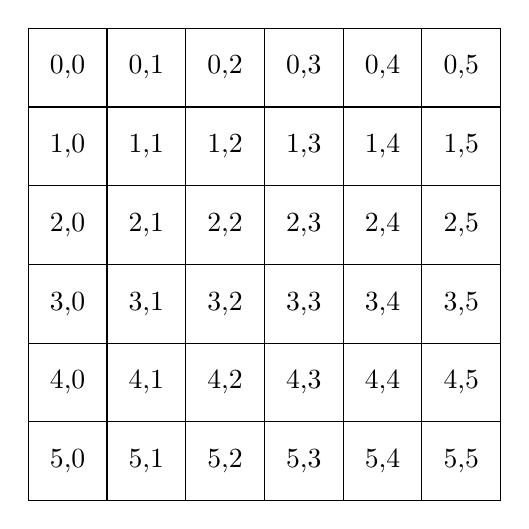
\begin{tikzpicture}[]
\foreach \x in {0,...,5}
\foreach \y in {0,...,5}
{
\draw (\x,-\y) +(.5,.5) rectangle ++(-.5,-.5);
\draw (\x,-\y) node{\y,\x};
}
\end{tikzpicture}}
\subfigure[Block (0,0) with 16 threads.]  
{  
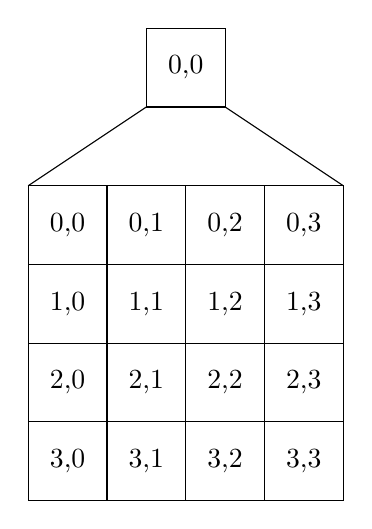
\begin{tikzpicture}[]
\foreach \x in {0,...,3}
\foreach \y in {0,...,3}
{
\draw (\x,-\y) +(.5,.5) rectangle ++(-.5,-.5);
\draw (\x,-\y) node{\y,\x};
}
\draw (1.5,2) +(.5,.5) rectangle ++(-.5,-.5);
\draw (1.5,2) node{0,0};
\draw[-] (2, 1.5) -- (3.5, 0.5);
\draw[-] (1, 1.5) -- (-0.5, 0.5);
\end{tikzpicture}}
\caption{Grid, blocks and threads.}
\label{fig:parallel}
\end{figure}

The smallest unit of work is a thread. Some amount of threads are contained within a block and blocks are arranged in a superstructure called a grid. From a programmer's perspective, threads of a block are executed in parallel and sharing memory between threads is possible and recommended. As the theoretical computational performance (for example $11.3 \cdot 10^{12}$ single-precision floating-point operations per second on an Nvidia GTX 1080 Ti) is much larger than the memory bandwidth (484.4 GB/s on Nvidia GTX 1080 Ti), a recommended strategy is to load data in parallel from the main memory to a block's shared memory and utilize this fast shared memory as much as possible in computations while minimizing the data stored in the main memory.

With CUDA, each of the threads runs the same function called a kernel with block and thread indices given as parameters. Each kernel call receives a unique set of block and thread indices, which can be used to decide which part of the problem the kernel solves to avoid overlapping computation.

\section{Algorithm \& Implementation} \label{section:algo}
In this section, we combine previously defined algorithms to form a full TSP solver. The main idea is to first preprocess the problem network to generate a candidate set using $\alpha$-nearness and to optimize the $\alpha$-values using subgradient optimization. The resulting candidate set is used to generate some initial tour candidates, which are then optimized by 2-opt to obtain a final candidate for an optimal tour.


\subsection{$\alpha$-nearness computation \& optimization} \label{section:alpopt}
After implementing the $\alpha$-value computation and optimization using the subgradient method on CPU, the computation of an MST during each of the subgradient optimization iterations was identified to be the most costly operation and the best candidate for parallel optimization. The CPU implementation uses Prim's algorithm to compute the MST, but for the parallel implementation, Boruvka's algorithm by \cite{401280} was chosen. In contrast to the serial computation in Prim's algorithm which adds a new vertex to the MST each iteration, Boruvka's algorithm connects multiple connected components of a graph during each iteration. Pseudocode for Boruvka's algorithm is presented in Algorithm \ref{boruvka}.

\begin{algorithm}[H]
	\caption{Parallel Boruvka} 
	\begin{algorithmic}[1]
		\State Initialize each vertex as a component of a graph without any edges.
	    \While {$|components| > 1$}
	    		\State Find a closest neighbor for each component.
	    		\State Remove cycles from edges found in previous step.
	    		\State Use pointer-doubling on all components to find which components to combine.
	    		\State Update components, degrees of the MST, and length of the MST.
	    \EndWhile
	\end{algorithmic} 
	\label{boruvka}
\end{algorithm}
Parallel implementation of Boruvka's algorithm is straightforward to implement from a high-level description of the algorithm, but some ideas such as pointer-doubling were used from \cite{gpumst}. The main computational bottleneck of the algorithm is on line 3 of Algorithm \ref{boruvka}, where we must loop through all of the $n^2$ pairs of vertices to find each component's nearest neighbor. For all pairs of indices $(i, j)$, the work is split so that each thread in a block of 64 threads loads a single value from range $j = blockIdx.y \cdot 64, \ldots, blockIdx.y \cdot 64 + 63$, respectively. Once all values are loaded, a thread calculates the minimal distance for all 64 pairs $i = threadIdx.x + blockIdx.x \cdot 64$ and $j = blockIdx.y \cdot 64, \ldots, blockIdx.y \cdot 64 + 63$ and saves it to shared memory. At the end of the kernel execution, the thread with index 0 loops through all the results saved by other threads in shared memory and commits them to global memory with atomic operations if they constitute a new global minimum for the component.

The following improvements to the previously stated algorithms are taken straight from \cite{HELSGAUN2000106}:
\begin{itemize}
	\item Instead of excluding one vertex and adding it later to the MST, the MST is computed first for all of the vertices, and an edge is added to one of the leaf vertices of the MST. The edge is chosen to be the longest second-shortest edge incident to a leaf vertex.
	\item The subgradient update rule is changed to $\pi^{k+1} = \pi^k + t^k(0.7 v^k + 0.3 v^{k-1})$, where $v^{-1} = v^0$.
	\item The step size $t^k$ stays constant for a fixed number of iterations called a period. The length of the first period is n/2 and the length of a period, as well as the step size, are halved each time a period ends.
	\item At the beginning, however, the step size is doubled until $W$ does not increase. Also, if the last iteration of a period leads to an increase of $W$, then the period length is doubled.
	\item The algorithm terminates when the step size, length of the period, or $v^k$ becomes zero.
\end{itemize}

The actual $\alpha$-value computation and the calculation of the last MST were done fully on the CPU because of their serial nature.

\subsection{Initial tour generation} \label{section:tourgen}
The initial tour generation is a simplified version of that presented in \cite{HELSGAUN2000106} we start with a random vertex and iteratively choose the next tour vertices. The next vertex is chosen from the candidate set associated with the current vertex, by the smallest $\alpha$-value. If multiple vertices share the same $\alpha$-value, ties are broken with the smallest cost in the original cost matrix. If all vertices from the candidate set are already chosen, the closest vertex not in the candidate list is selected. Randomly choosing the first vertex seems to induce enough randomness to generate diverse-enough tour candidates.

\subsection{2-opt}
In addition to the non-restricted 2-opt variant described above, we also evaluate an improvement to the algorithm used in the original Lin-Kernighan heuristic. The improvement made by \cite{linkernighan} is as follows: if we denote the edges removed in a $\lambda$-opt operation with $(x_1, x_2, \ldots, x_{\lambda})$ and the edges replacing them as $(y_1, y_2, \ldots, y_{\lambda})$, then each $y_i$ should belong to the candidate set. In theory, this should lead to a better runtime, as there are fewer edges to check each iteration, and to a better quality solution because there are fewer local minima in which to get stuck.

For the unrestricted variant, the kernel is very similar to that in Section \ref{section:alpopt}. The problem is the same, as the algorithm must loop through all of the $n^2$ pairs of vertices and find a minimum. The improved variant is more difficult to effectively parallelize, as the candidate set is spread around the whole tour. Only modest speedups are made compared to a CPU implementation with having each thread looping through a vertex's candidate set and committing the minimum to global memory if necessary. 

The CPU implementation includes some parallel optimization to make the comparison more relevant. The outer-loop of the 2-opt is parallelized between cores available on the machine so that each core gets approximately the same amount of work. This is done using the OpenMP by \cite{openmp}. 

\section{Results} \label{section:res}
The experiments were conducted on the author's computer with the following hardware specifications: Intel i7-8700k processor at 4.8GHz, 32GB 3200MHz DDR4 memory, and Nvidia GTX 1080 Ti GPU.

4 different variations of the algorithm are compared, each evaluated 100 times with different random starting tours.
\begin{enumerate}
	\item (RAND) Random tour initialization with normal 2-opt.
	\item (ALPHA1) $\alpha$-value initial tour generation as in Section \ref{section:tourgen}, with normal 2-opt.
	\item (ALPHA2) $\alpha$-value initial tour generation as in Section \ref{section:tourgen}, with 2-opt restricted to candidate set edges.
	\item (ALPHA3) $\alpha$-value initial tour generation as in Section \ref{section:tourgen}, with 2-opt restricted to candidate set edges, followed by normal 2-opt.
\end{enumerate}

2D euclidean instances from TSPLIB by \cite{Rein91} were used as benchmark instances and all algorithms were run with a candidate set size of 10.

\subsection{Solution quality}
We measure solution quality only on the GPU-variants of the algorithm, as the CPU implementations have similar performance but are just slower. The results are detailed in Table \ref{resqual}, where an asterisk (*) after the optimum denotes that the value is an upper bound for an optimum solution. 

\begin{table}[H]
\centering
\begin{tabular}{@{}llllll@{}}
\toprule
Instance & RAND    & ALPHA1 & ALPHA2  & ALPHA3 & Optimum \\ \midrule
eil101   & 680     & \textbf{668}    & 739     & 669    & 629     \\
a280     & 2864    & \textbf{2748}   & 3239    & 2751   & 2579    \\
att532   & 94720   & 91159  & 108755  & \textbf{90857}  & 86729   \\
pr1002   & 283706  & \textbf{271534} & 322240  & 272928 & 259045  \\
d1291    & 59736   & 53835  & 58693   & \textbf{53350}  & 50801   \\
d1655    & 71483   & \textbf{65789}  & 75145   & 65944  & 62128   \\
d2103    & 93343   & 82268  & 87406   & \textbf{82127}  & $80450^*$   \\
pcb3038  & 155614  & 145993 & 167543  & \textbf{145544} & 137694  \\
rl5915   & 682396  & 606610 & 680485  & \textbf{602801} & $565530^*$ \\
rl11849  & 1091468 & \textbf{982572} & 1122952 & 982636 & $923307^*$  \\ \bottomrule
\end{tabular} 
\caption{Best results for each algorithm, with best overall bolded.} \label{resqual}
\end{table}

As can be seen from Table \ref{resqual}, variants ALPHA1 and ALPHA3 perform quite similarly and considerably better than ALPHA2 and RAND variants. The worse performance of ALPHA2 came as a bit of a surprise because of the results of \cite{HELSGAUN2000106}, which are consistently better with a small candidate sets applied to $\lambda$-opt. The worse results might be due to the use of only 2-opt in this solver, as the LKH uses a 5-opt move as its base move. Table \ref{table:reserr} details the errors as percentage distances from the optimum values.

\begin{table}[H]
\centering
\begin{tabular}{@{}lllll@{}}
\toprule
Instance & RAND  & ALPHA1 & ALPHA2 & ALPHA3 \\ \midrule
eil101   & 8.1   & 6.2    & 17.5   & 6.4    \\
a280     & 11.1  & 6.6    & 25.6   & 6.7    \\
att532   & 9.2 & 5.1  & 25.4  & 4.8  \\
pr1002   & 9.5   & 4.8    & 24.4   & 5.4    \\
d1291    & 17.6  & 6.0    & 15.5   & 5.0    \\
d1655    & 15.1  & 5.9    & 21.0   & 6.1    \\
d2103    & 16.0  & 2.3    & 8.6    & 2.1    \\
pcb3038  & 13.0  & 6.0    & 21.7   & 5.7    \\
rl5915   & 20.7  & 7.3    & 20.3   & 6.6    \\
rl11849  & 18.2  & 6.4    & 21.6   & 6.4    \\ \midrule
Average error & 13.9 & 5.7    & 20.2   & 5.5 \\\bottomrule
\end{tabular}
\caption{Errors of the algorithms from the optimal values as percentage distances.} \label{table:reserr}
\end{table}

The considerably lower error percentages of the $\alpha$-value calculation augmented algorithms demonstrate the usefulness of the $\alpha$-measure. The impact of the $\alpha$-measure is especially visible on larger instances, in which a normal 2-opt has a huge number of local minima in which it can get stuck, thus leading to large error percentages. $\alpha$-value based methods are able to circumvent most of these local minima to achieve significantly lower error percentages.

\subsection{Efficiency}
The running time for all four variants of the algorithms is measured in milliseconds on both CPU and GPU, and the computation times are presented in Table \ref{table:eff3}. The average running time is calculated on instances between eil101 to pcb3038 in order to compare the efficiency of all GPU and CPU algorithms on average.

\begin{table}[H]
\begin{adjustbox}{center}
\begin{tabular}{@{}lllllllll@{}}
\toprule
Instance & \begin{tabular}[c]{@{}l@{}}RAND\\ GPU\end{tabular} & \begin{tabular}[c]{@{}l@{}}ALPHA1\\ GPU\end{tabular} & \begin{tabular}[c]{@{}l@{}}ALPHA2\\ GPU\end{tabular} & \begin{tabular}[c]{@{}l@{}}ALPHA3\\ GPU\end{tabular} & \begin{tabular}[c]{@{}l@{}}RAND\\ CPU\end{tabular} & \begin{tabular}[c]{@{}l@{}}ALPHA1\\ CPU\end{tabular} & \begin{tabular}[c]{@{}l@{}}ALPHA2\\ CPU\end{tabular} & \begin{tabular}[c]{@{}l@{}}ALPHA3\\ CPU\end{tabular} \\ \midrule
eil101   & 454                                                & 275                                                  & 231                                                  & 298                                                  & 91                                                 & 125                                                  & 107                                                  & 109                                                  \\
a280     & 1020                                               & 633                                                  & 493                                                  & 614                                                  & 718                                                & 984                                                  & 772                                                  & 1376                                                 \\
att532   & 2219                                               & 1578                                                 & 1297                                                 & 1631                                                 & 5339                                               & 6080                                                 & 5006                                                 & 5602                                                 \\
pr1002   & 6743                                               & 5797                                                 & 3824                                                 & 4424                                                 & 39628                                              & 25900                                                & 21410                                                & 23377                                                \\
d1291    & 7088                                               & 7268                                                 & 6956                                                 & 7409                                                 & 95540                                              & 45515                                                & 40319                                                & 46100                                                \\
d1655    & 11102                                              & 13555                                                & 12222                                                & 14298                                                & 197076                                             & 104244                                               & 89109                                                & 98342                                                \\
d2103    & 14706                                              & 19822                                                & 19082                                                & 19785                                                & 367981                                            & 140303                                               & 126630                                               & 139569                                               \\
pcb3038  & 24887                                              & 52771                                                & 49327                                                & 54765                                                & 1085717                                                    & 579399                                                      & 520704                                                      & 730849                                                     \\
rl5915   & 125805                                             & 198356                                               & 188176                                               & 198295                                               &                                                    &                                                      &                                                      &                                                      \\
rl11849  & 913566                                             & 1084582                                              & 1026429                                              & 1046155                                              &                                                    &                                                      &                                                      &                                                      \\ \midrule
Average & 8527 & 12712 & 11679 & 12903 & 224011 & 112818 & 100507 & 130665 \\ \bottomrule
\end{tabular}
\end{adjustbox}
\caption{Combined running times for all algorithms in milliseconds.} \label{table:eff3}
\end{table}

While small instances are still faster with CPU implementaions, as can be seen in Table \ref{table:eff3}, GPU implementations are significantly faster on average. Larger instances were not even computed with CPU implementations, as the running time became excessively large. To illustrate the speedup better, Figure \ref{fig:effn} shows how the algorithms scale as a function of instance size.

\begin{figure}[H]
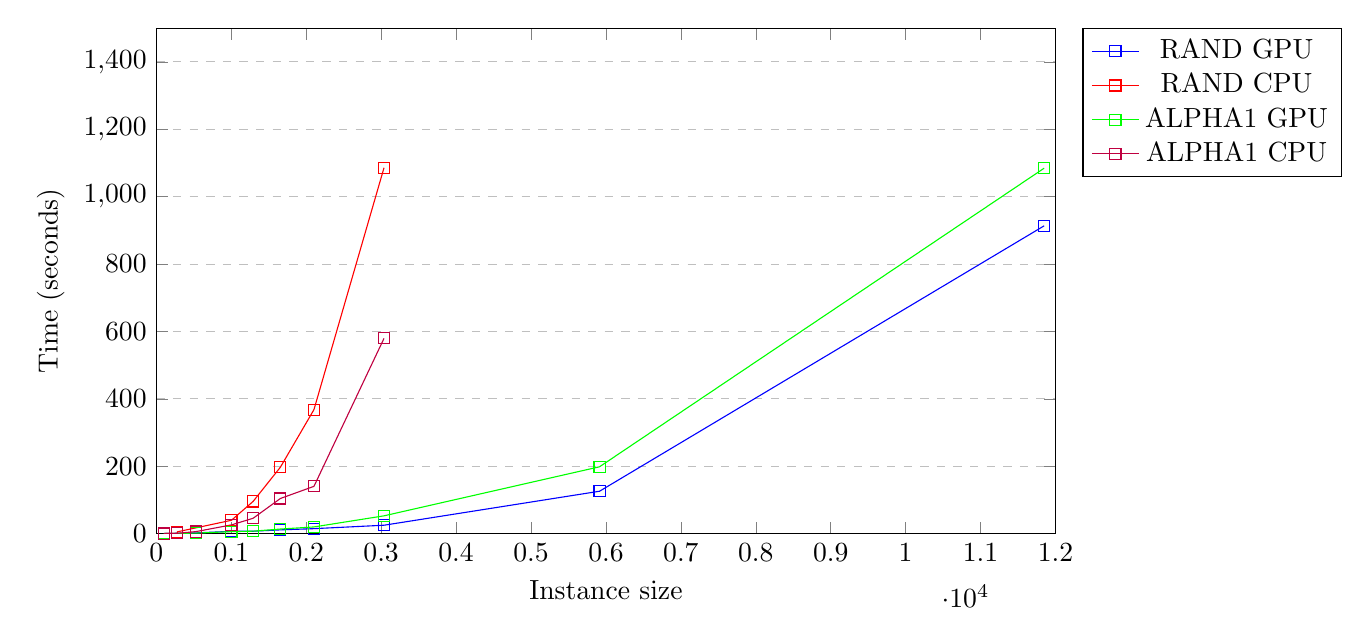
\begin{tikzpicture}
\begin{axis}[
    xlabel={Instance size},
    ylabel={Time (seconds)},
    xmin=0, xmax=12000,
    ymin=0, ymax=1500,
    height=8cm, width=13cm,
    xtick={},
    ytick={},
    legend pos=outer north east,
    ymajorgrids=true,
    grid style=dashed,
]

\addplot[
    color=blue,
    mark=square,
    ]
    coordinates {
    (101, 0.454)(280, 1.020)(532, 2.219)(1002, 6.743)(1291, 7.088)(1655, 11.102)(2103, 14.706)(3038, 24.887)(5915, 125.805)(11849, 913.566)
    };
    \legend{RAND GPU, RAND CPU, ALPHA1 GPU, ALPHA1 CPU}
\addplot[
    color=red,
    mark=square,
    ]
    coordinates {
    (101, 0.091)(280, 0.718)(280, 5.339)(1002, 39.628)(1291, 95.540)(1655, 197.076)(2103, 367.981)(3038, 1085.717)
    };
    
    \addplot[
    color=green,
    mark=square,
    ]
    coordinates {
    (101, 0.275)(280, 0.633)(532, 1.578)(1002, 5.797)(1291, 7.268)(1655, 13.555)(2103, 19.822)(3038, 52.771)(5915, 198.356)(11849, 1084.582)
    };
\addplot[
    color=purple,
    mark=square,
    ]
    coordinates {
    (101, 0.125)(280, 0.984)(532, 6.08)(1002, 25.9)(1291, 45.515)(1655, 104.244)(2103, 140.3)(3038, 579.4)
    };
    
\end{axis}
\end{tikzpicture} 
\caption{RAND and ALPHA1 solver computation times as a function of instance size.} \label{fig:effn}
\end{figure}

The scaling of the CPU-variants is much steeper, with GPU implementations capable of solving 5-times larger instances than the CPU implementations in a similar amount of time. These results were expected, as CPUs can traditionally handle 4-16 tasks at the same time, but modern GPUs can concurrently handle thousands of threads. As all ALPHA-variants have very similar timings, the plot only shows ALPHA1. The speedups are especially visible in the largest instance solved with CPU implementations, which is detailed in Figure \ref{fig:effbar}.

\begin{figure}[H]
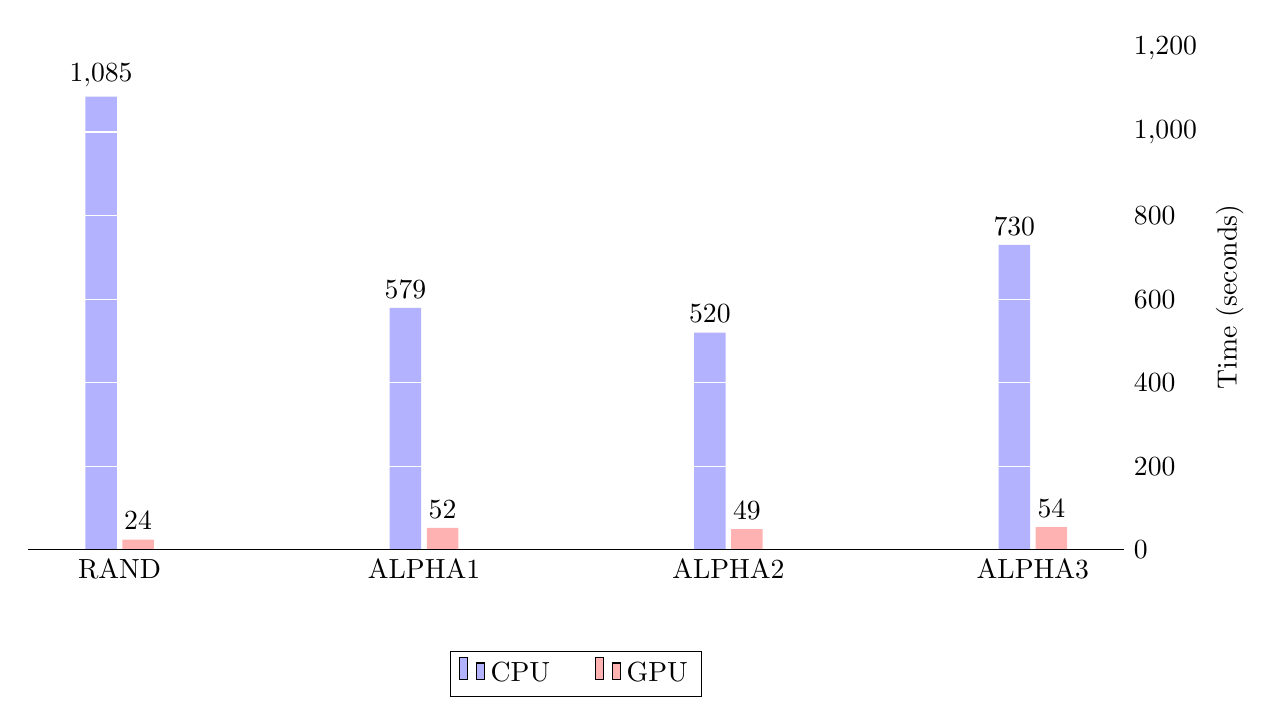
\begin{tikzpicture}
  \centering
  \begin{axis}[
        ybar, axis on top,
        title={},
        height=8cm, width=15.5cm,
        bar width=0.4cm,
        ymajorgrids, tick align=inside,
        major grid style={draw=white},
        enlarge y limits={value=.1,upper},
        ymin=0, ymax=1100,
        axis x line*=bottom,
        axis y line*=right,
        y axis line style={opacity=0},
        tickwidth=0pt,
        enlarge x limits=true,
        legend style={
            at={(0.5,-0.2)},
            anchor=north,
            legend columns=-1,
            /tikz/every even column/.append style={column sep=0.5cm}
        },
        ylabel={Time (seconds)},
        symbolic x coords={
           RAND, ALPHA1, ALPHA2, ALPHA3},
       xtick=data,
       nodes near coords={
        \pgfmathprintnumber[precision=0]{\pgfplotspointmeta}
       }
    ]
    \addplot [draw=none, fill=blue!30] coordinates {
      (RAND,1085)
      (ALPHA1,579) 
      (ALPHA2,520)
      (ALPHA3,730)  };
   \addplot [draw=none,fill=red!30] coordinates {
      (RAND,24)
      (ALPHA1,52) 
      (ALPHA2,49)
      (ALPHA3,54) };

    \legend{CPU, GPU}
  \end{axis}
  \end{tikzpicture} \caption{Running times for instance pcb3038 in seconds.}
  \label{fig:effbar}
\end{figure}

On pcb3038-instance, the GPU RAND is 40 times faster than the CPU counterpart. The GPU ALPHA algorithms also beat their counterparts by a factor of 10. Tables \ref{fig:eff1} and \ref{fig:eff2} in the Appendix details the running times for both the preprocessing (subgradient optimization and $\alpha$-values) and 2-opt in milliseconds.

\section{Conclusions} \label{section:concl}
This thesis aimed to identify effective places for parallelization in the algorithms underlying the state-of-the-art TSP solver LKH. Parallel programming was applied to the 2-opt algorithm and $\alpha$-nearness subgradient optimization, gaining speedups of up to 10--40 times for the GPU implementations over the CPU ones. The effectiveness of $\alpha$-nearness as a measure for candidate set generation was also verified, and the solutions obtained by the parallel GPU algorithms achieved significantly better results compared to standard implementations, with respect to optimal solution costs. Based on the results of this thesis, a parallel implementation of a state-of-the-art solver, such as the LKH, could offer considerable gains in computation time.


\bibliography{tsp}

\section{Appendix}
\begin{table}[H]
\centering
\begin{tabular}{@{}llllllll@{}}
\toprule
Instance & \begin{tabular}[c]{@{}l@{}}RAND\\ 2-opt\end{tabular} & \begin{tabular}[c]{@{}l@{}}ALPHA1\\ 2-opt\end{tabular} & \begin{tabular}[c]{@{}l@{}}ALPHA1\\ prep.\end{tabular} & \begin{tabular}[c]{@{}l@{}}ALPHA2\\ 2-opt\end{tabular} & \begin{tabular}[c]{@{}l@{}}ALPHA2\\ prep.\end{tabular} & \begin{tabular}[c]{@{}l@{}}ALPHA3\\ 2-opt\end{tabular} & \begin{tabular}[c]{@{}l@{}}ALPHA3\\ prep.\end{tabular} \\ \midrule
eil101   & 454                                                  & 92                                                     & 183                                                    & 53                                                     & 178                                                    & 113                                                    & 185                                                    \\
a280     & 1020                                                 & 336                                                    & 297                                                    & 200                                                    & 293                                                    & 323                                                    & 291                                                    \\
att532   & 2219                                                 & 1008                                                   & 570                                                    & 731                                                    & 566                                                    & 1081                                                   & 550                                                    \\
pr1002   & 6743                                                 & 3322                                                   & 2475                                                   & 2507                                                   & 1317                                                   & 3167                                                   & 1257                                                   \\
d1291    & 7088                                                 & 5284                                                   & 1984                                                   & 4930                                                   & 2026                                                   & 5424                                                   & 1985                                                   \\
d1655    & 11102                                                & 9944                                                   & 3611                                                   & 8995                                                   & 3227                                                   & 10084                                                  & 4214                                                   \\
d2103    & 14706                                                & 14426                                                  & 5396                                                   & 13655                                                  & 5427                                                   & 14391                                                  & 5394                                                   \\
pcb3038  & 24887                                                & 35433                                                  & 17338                                                  & 32028                                                  & 17299                                                  & 34484                                                  & 20281                                                  \\
rl5915   & 125805                                               & 152106                                                 & 46250                                                  & 142345                                                 & 45831                                                  & 152962                                                 & 45333                                                  \\
rl11849  & 913566                                               & 764269                                                 & 320313                                                 & 700677                                                 & 325752                                                 & 742629                                                 & 303526                                                 \\ \bottomrule
\end{tabular} 
\caption{Execution times for GPU-variants in milliseconds.} \label{fig:eff1}
\end{table}

\begin{table}[H]
\begin{tabular}{@{}llllllll@{}}
\toprule
Instance & \begin{tabular}[c]{@{}l@{}}RAND\\ 2-opt\end{tabular} & \begin{tabular}[c]{@{}l@{}}ALPHA1\\ 2-opt\end{tabular} & \begin{tabular}[c]{@{}l@{}}ALPHA1\\ prep.\end{tabular} & \begin{tabular}[c]{@{}l@{}}ALPHA2\\ 2-opt\end{tabular} & \begin{tabular}[c]{@{}l@{}}ALPHA2\\ prep.\end{tabular} & \begin{tabular}[c]{@{}l@{}}ALPHA3\\ 2-opt\end{tabular} & \begin{tabular}[c]{@{}l@{}}ALPHA3\\ prep.\end{tabular} \\ \midrule
eil101   & 91                                                   & 49       & 76       & 38       & 69       & 39       & 70       \\
a280     & 718                                                  & 286      & 698      & 246      & 526      & 875      & 501      \\
att532   & 5339                                                 & 1672     & 4408     & 906      & 4100     & 1522     & 4080     \\
pr1002   & 39628                                                & 7544     & 18356    & 3063     & 18347    & 5316     & 18061    \\
d1291    & 95540                                                & 12337    & 33178    & 5194     & 35125    & 11625    & 34475    \\
d1655    & 197076                                               & 24490    & 79754    & 9110     & 79999    & 19204    & 79138    \\
d2103    & 367981                                               & 32074    & 108229   & 17350    & 109280   & 30566    & 109003   \\
pcb3038  & 1085717                                              & 132144   & 447255   & 35963    & 484741   & 244017   & 486832   \\ \bottomrule
\end{tabular}
\caption{Execution times for CPU-variants in milliseconds.} \label{fig:eff2}
\end{table}


\end{document}
